\def\be{\begin{equation}}
\def\ee{\end{equation}}

\documentclass[12pt]{article}
\usepackage{graphicx}
\usepackage{notoccite}
\usepackage{epigraph} % epigraph
\usepackage{float}

\usepackage[square, numbers, comma, sort&compress]{natbib}  % Use the "Natbib" style for the references in the Bibliography
\usepackage{verbatim,listings}  % Needed for the "comment" environment to make LaTeX comments
\usepackage{array}  % Needed for the "comment" environment to make LaTeX comments
\usepackage{vector}  % Allows "\bvec{}" and "\buvec{}" for "blackboard" style bold vectors in maths

% \documentclass[a4paper,12pt]{article}
%\usepackage[a4paper,vmargin={20mm,20mm},hmargin={20mm,20mm}]{geometry}
\usepackage{amsmath,amsfonts,amsthm,color,psfrag,epsf,graphicx}
% \usepackage{pstricks}
\usepackage{enumerate,caption}
%\usepackage[lined,algonl,boxed]{algorithm2e}
\usepackage[ruled,linesnumbered,vlined]{algorithm2e}
\usepackage{float}
% \SpecialCoor
\def\subsum{\mathit{\Sigma}}




\def\ifthesis{\iftrue}
\setcounter{secnumdepth}{2}
\newenvironment{myindentpar}[1]%
{\begin{list}{}%
         {\setlength{\leftmargin}{#1}}%
         \item[]%
}
{\end{list}}




\graphicspath{{Figures/}}  % Location of the graphics files (set up for graphics to be in PDF format)
\usepackage{epigraph} % epigraph
%customize: \setlength{\epigraphwidth}{7cm}\setlength{\epigraphrule}{0pt}
%use: \epigraph{text}{reference}

%customize: \setlength{\epigraphwidth}{7cm}\setlength{\epigraphrule}{0pt}
%use: \epigraph{text}{reference}
\begin{document}
%\bibliographystyle{iopart-num}
\bibliographystyle{unsrt}
%\chapter{Particle In cell} % Write in your own chapter title
%label{Chapter3}
%\lhead{Chapter 3. \emph{A Chapter}} % Write in your own chapter title to set the page header
\section{Introduction}
%Maybe add in the advanced probe section
%Mention somehwere that Ti = Te is a an assumption relied upon because of the difficutly to get Ti measurements. Mention why you can't use standard Lp to get Ti measurements. Talk about difficulties in obtaining plasma potential too then introduce advanced probes 
%
% http://iopscience.iop.org/article/10.1088/1742-6596/666/1/012001/pdf
%
%Talk about the debye sheath and MPS only applies above critical angle
%Stangeby fluid code
%http://iopscience.iop.org/article/10.1088/0029-5515/52/8/083012/meta
%\cite{MPS-Stangeby}
%kinetic code confirming Stangeby fluid stuff
%http://iopscience.iop.org/article/10.1088/0741-3335/58/2/025008/meta


%Riemann then goes further to generalise the Bohm criterion with finite T_i and introduees the gamma factor infront of Ti 
%http://iopscience.iop.org/article/10.1088/0022-3727/24/4/001/meta

Langmuir probes are the oldest type of plasma diagnostic device and are still one of the most frequently employed tools used to obtain information about conditions inside a plasma. In relation to tokamaks, Langmuir probes are the most reported edge diagnostic in the literature \cite{matthews}.The main advantage of using probes is that they can make highly localised measurements, almost all other diagnostics give volume averaged measurements. Readings from Langmuir probes are an essential input into simulation codes that aim to simulate the edge region of a tokamak, as the probes measure plasma conditions at solid surfaces, which is typically the most important output from modelling codes. These codes require inputs with high spatial and temporal resolution \cite{first_wall}. The probes take their name from the Nobel prize winning scientist Irving Langmuir who coined the term plasma and whose paper published in 1926 with H.M. Mott-Smith provided a means to measure plasma parameters by obtaining a Current-Voltage curve (IV curve) using a probe \cite{mottsmith}. The probe in its simplest form is a metallic electrode, electrically biased with respect to a reference electrode which is then inserted into a plasma to draw an ion or electron current. %In the simplest case the electrode has a well defined geometry either planar, spherical or cylindrical. %This set-up is known as the single probe. More sophisticated  designs do exist such as double and triple probes and will be discussed later in this report.
Electrical probes are used to diagnose a wide range of plasmas from space plasmas with low-density and weak magnetic fields to those at the edge of nuclear fusion devices with hostile conditions to material surfaces and strong magnetic fields. The use of probes requires direct contact to be made between the probe and the plasma and so their use is limited by the conditions in which they can survive. This restricts the use of probes to the edge of tokamak devices where the plasma is less dense and cooler. 
\paragraph{}
Langmuir probes are a powerful diagnostic capable of providing local measurements of the plasma potential $(V_{p})$, electron density $(n_e)$ and electron temperature $(T_e)$ with a good time resolution of approximately $10^{-3}$ seconds \cite{probetheoryandpractise}. They are fairly easy both to design and build and acquiring data from them is straightforward. Despite their simplicity in construction and operation, probes do have a downside compared to other diagnostics. As probes are in contact with the plasma, they perturb it, changing the local density and potential in the surrounding plasma. This complicates the interpretation of probe data. The role of probe theory is to determine the unperturbed values of the plasma which would exist in the absence of the probe. However theoretical models used to interpret the data can be very complicated and in some cases non-existent. No general model exists that is capable of relating the measured current voltage curves with the actual plasma properties under all possible physical conditions. An overview of the general probe method will be given followed by complications that arise, specifically in the presence of magnetic fields. 


%"The measurement resolution requirements are set in
%part by the needs of simulation codes. The electron tem-
%perature Te ~r! and density ne ~r! profiles are needed with
%1- to 2-mm spatial resolution ~less than the 10- to 15-mm
%profile decay length! to define SOL and pedestal profiles.
%Poloidal electric field Eo ~r! and radial electric Er ~r! pro-
%files are needed to define radial and poloidal drifts. Pro-
%files of fluctuation levels in density ne , poloidal and radial
%electric fields Eo ~r! and Er ~r!, and electron temperature
%Te , with bandwidth of up to 3 to 5 MHz and spatial
%resolution of 1 to 2 mm are needed to evaluate turbulent
%components of particle and heat transport and other ef-
%fects such as Reynolds Stress."   http://epubs.ans.org/?a=1682

\section{Sheath Physics}
 

In order to understand particle collection by a Langmuir probe it is essential to realise the role played by the plasma sheath. An electrostatic sheath forms whenever a material object comes into contact with a plasma. %, for example, a Langmuir probe inserted into the plasma or tiles in the divertor region of a tokamak. 
The sheath dominates the transport of ions and electrons to the material surface. The difference in mobility between electrons and ions is the foundation for the formation of a sheath. For example, consider the case of a divertor tile coming into contact with plasma. Before contact with the plasma, there is no net charge on the tile, the tile is neutral. As the plasma reaches the tile, electrons in the plasma will rush to the tile ahead of the ions. This occurs because electrons are much less massive than ions and so move around much faster in the plasma. This process can not go on indefinitely. A net negative charge builds up on the tile which leads to the formation of a potential barrier. This barrier repels electrons and attracts ions \cite{sheathformation}. The potential barrier continues to increase, reducing the electron flux until a steady state is obtained once the electron flux becomes equal to the ion flux. The potential of the tile at steady state is the floating potential $V_F$. The tile is said to be floating. The potential a floating object reaches depends on the plasma potential, the temperature of the electrons and ions and the mass ratio of the charged particles. This will be derived in section  \ref{section:Ideal}.
\begin{figure}[H]
\centering
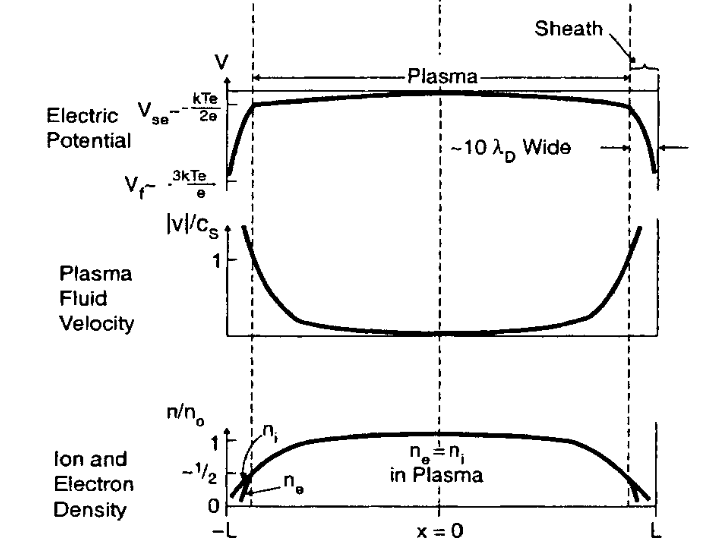
\includegraphics[width=0.8\textwidth]{sheath.png}
\caption{A schematic of the variation of electric potential, plasma velocity and particle density with distance from the wall in a plasma \cite{stangeby-sheath}.}
\label{fig:stangebysheath}
\end{figure} 
The floating tile is a region of charge in an otherwise quasineutral plasma. The behaviour of the plasma in response to the presence of this charge is governed by the Poisson equation
\be
\nabla^2 \psi = - \frac{e}{\epsilon_0}(n_i - n_e)
\label{eq:Poisson}
\ee 
where $\psi$ is the potential at a given point in the plasma, $e$ the electron charge, $n_i$ the ion density, assuming singly charged ions and $n_e$ the electron density. The electrons mobility allows them to react quickly to the charge and they adopt a Boltzmann distribution 
\be 
n_e = n_{\infty} \exp \left( \frac{e \psi}{T_e} \right)
\label{eq:Boltzmann}
\ee
where $n_{\infty}$ is the plasma density, for both electrons and ions, far from the external charge and $T_e$ is the electron temperature. Over fast timescales the ions can be considered stationary. Substituting equation \ref{eq:Boltzmann} into equation \ref{eq:Poisson} gives 
\be 
\nabla^2 \psi = -\frac{e n_i}{\epsilon_0}\left(1 - \exp \left(\frac{e \psi}{T_e} \right) \right)
\ee
By expanding the exponential term and asssuming $T_e >> e \psi$ we find 
\be 
\nabla^2 \psi \approx \frac{e^2 n_i}{\epsilon_0 T_e} \psi = \frac{\psi}{\lambda_D ^2}
\label{eq:debye}
\ee
where $\lambda_D$ is the Debye length. Expanding equation \ref{eq:debye} we find
\be 
\psi = \psi_0 \exp \left(-\frac{x}{\lambda_D} \right)
\ee 
the potential of the charge drops off exponentialy with distance into the plasma. The Debye length is then the distance over which the charge can penetrate into the plasma. This thin layer where the potential from the charge is able to influence the plasma is known as the sheath. The sheath is a transition layer in the plasma between an external charge and the bulk plasma. In the sheath, quasi-neutrality no longer holds. %, the plasma gains a positive space charge as ions are attracted towards the negative potential and the electrons repelled.
The sheath acts to shield the rest of the plasma from the external charge. In the case of a negatively floating tile, the potential from the tile will be contained in the sheath region. Ions are accelerated in the sheath towards the tile while the electrons are de-accelerated. % Assuming the ions are cold, any kinetic energy they gain in the sheath will be in the form of lost potential energy. Applying conservation of energy we can then write 
%\be 
%\frac{1}{2} m_i v^2 = -e \psi
%\ee
%So the velocity of an ion at a given point in the sheath is determined by the potential 
%\be 
%|v_i| = \left( -\frac{2eV}{m_i} \right)^{1/2}
%\ee
%From particle conservation we know that at any point in the sheath 
%\be 
%n_i v_i = n_s v_s  \rightarrow n_i = \frac{n_s v_s}{v_i} = n_s v_s \left(-\frac{m_i}{2eV}\right)^{1/2}
%\ee 
%where $s$ denotes values at the sheath entrance. Applying Poissons equation in the sheath we find
%\be 
%\nabla ^2 \psi = - \frac{e}{\epsilon_0} \left(n_i - n_{\infty} \exp \left[ \frac{e(V-V_s)}{T_e} \right] \right) = -\frac{e}{\epsilon_0} 
%\ee 
%where $V_s$ is the potential of the plasma at the sheath entrance. 
In order for the sheath to be stable, the ions must enter the sheath with sufficient velocity such that $v \geq c_s$ where $c_s$ is the plasma sound speed. This is the well known Bohm Criterion \cite{bohm}. It is possible to derive this result by considering a 1D, unmagnetised plasma in contact with a material surface as shown in figure \ref{fig:stangebysheath}. In the bulk plasma the plasma potential is zero. We assume the ions are born stationary and cold, far from the tile, in the bulk plasma. It is assumed the electrons have a Maxwellian distribution so that their density profile can be described by the Boltzmann relation
\be
n_e = n_{se} e^{\frac{e(V-V_{se})}{KT_e}}
\label{eq:ne}
\ee
where $n_{se}$ is the electron density at the sheath entrance, $V_{se}$ the plasma potential at the sheath entrance, $K$ the Boltzmann constant and $T_e$ the electron temperature in Kelvin. This is a valid approximation as most electrons are reflected in the sheath and so the Maxwellian distribution is maintained. There is a potential drop between the bulk plasma and the sheath entrance, in other words, $V_{se}$ is negative relative to the plasma potential. This potential drop occurs in a region of plasma known as the pre-sheath. It is this drop in potential that accelerates the ions so that they satisfy the Bohm Criterion. For the ions we apply conservation of energy which leads to 
\be 
\frac{1}{2} m_i v^2 = - e \psi 
\ee 
This equation is valid at all points in the plasma.
From particle conservation, in the absence of sources and sinks, we have 
\be 
n_i v_i =  n_{se} v_{se} \rightarrow n_i =  \frac {n_{se} v_{se}}{v_i}
\label{eq:particle_conservation}
\ee 
From energy conservation we have 
\be 
v_{se} = \left( -\frac{2e\psi_{se}}{m_i} \right) ^{1/2} \hspace{2cm}  v_{i} = \left( -\frac{2e\psi}{m_i} \right) ^{1/2}
\label{eq:velocities}
\ee
Plugging this into equation \ref{eq:particle_conservation} gives 
\be
n_i = n_{se}\left(\frac{\psi_{se}}{\psi} \right) ^{1/2}
\label{eq:ni}
\ee
Substituting equations \ref{eq:ni} and \ref{eq:ne}, for the ion density and electron density respectively, into Poissions equation, equation \ref{eq:Poisson} and we get
\be 
\frac{d^2 \psi}{d x^2 } = -\frac{e}{\epsilon_0} n_{se} \left[ \left(\frac{\psi_{se}}{\psi}\right)^{1/2} - \exp\left[\frac{e(\psi -\psi_{se})}{kT_e}\right] \right]
\label{eq:Poisson_subbed}
\ee
This is valid in both the bulk plasma and the sheath. We now define a variable $\Delta$ such that
\be 
\Delta = \psi_{se} - \psi
\label{eq:Delta}
\ee
In the sheath region $\psi < \psi_{se}$ therefore $\Delta >0$. We can now carry out an expansion of the two terms on the right hand side of equation \ref{eq:Poisson_subbed}.
\be 
\left(\frac{\psi_{se}}{\psi}\right) ^{1/2}  = \left(\frac{\Delta}{\psi} +1 \right) \approx 1 + \frac{\Delta}{2\psi} = 1 - \frac{\Delta}{2 |\psi_{se}|}
\label{eq:psi_subbed}
\ee
Here we take a point just inside the sheath such that $\psi \approx \psi_{se}$. 
The second substitution and expansion gives 
\be
\exp\left[\frac{e(\psi - \psi_{se})}{kT_e} \right] =  \exp\left[\frac{-e\Delta}{kT_e} \right] \approx 1 - \frac{e \Delta}{k T_e}
\label{eq:exp_sub}
\ee
We can now substitute equations \ref{eq:Delta},\ref{eq:psi_subbed} and \ref{eq:exp_sub} into equation \ref{eq:Poisson_subbed}. 
\be
\frac{d^2 \Delta}{d x^2}  = \frac{e}{\epsilon_0} n_{se} \left[\frac{e \Delta}{k T_e} - \frac{\Delta}{2 |\psi_{se}|} \right]
\ee
This will only provide non-oscillatory solutions when 
\be 
\frac{e}{k T_e} \geq \frac{1}{2 |\psi_{se}|}
\ee 
Which, with the use of equation \ref{eq:velocities} can be recast as 
\be 
v_{se} \geq \sqrt{\frac{k T_e}{m_i}}
\ee
which is the Bohm criterion with $c_s = \sqrt{\frac{k T_e}{m_i}}$. 
Ions are accelerated in the pre-sheath which penetrates deep into the plasma. In deriving this value for $c_s$ it was assumed that the ions are cold. By relaxing this assumption and having ions with a finite temperature, a new value for the sound speed can be obtained \cite{stangeby-2000} 
\be
c_s = \sqrt{\frac{k(T_e + T_i)}{m_i}}
\ee

%
% The sheath has a thickness on the order of 10 Debye lengths which corresponds to $\approx $ 10$ \mu m$ in a typical scrape off layer off a tokamak. % EXPLAIN DEBYE LENGTH, GET FORMULA, 
% It is possible to calculate the ion velocity at any point in the sheath by applying the principle of conservation of energy as demonstrated in this simple model.
%
%For simplicity we will work in one dimension. The bulk plasma lies at the origin x=0, here quasi-neutrality holds and the potential $V=0$. The floating material surface lies at x=b and has a negative potential with respect to the plasma. 
%By applying conservation of energy we know that the velocity of the ions $v(x)$ at any position is given by 
%\be 
%v(x) = v_0 \sqrt{1 - \frac{2 e V(x)}{m_i v_0^2}}
%\ee
%where $v_0$ is the initial velocity of the ions before entering the sheath and $m_i$ is the mass of the ions. 
%
%The moving ions form an electric current density  
%\be 
%J_i = e n(x) v(x) = e n_0 v_0 
%\ee
%This is conserved so doesn't vary with position in the sheath. As a result of this the density of ions must decrease as we move in to the sheath to balance out the increase of speed as the ions accelerate towards the negative charge. The density in the sheath is given by 
%\be 
%n(x) = \frac{n_0 v_0 }{v(x)} = \frac{n_0}{\sqrt{1 - \frac{2 e V(x)}{m_i v_0^2}}}
%\ee 
%Assuming a Maxwellian distribution of electrons the electron density in the sheath is then described by the Boltzmann equation 
%\be
%n_e(x) = n_0 \exp \left(\frac{e V(x)}{k T_e}\right)
%\label{eq:sheathdense}
%\ee
%This is an often used approximation as most electrons in the sheath are reflected by the negative wall and so oscillate back and forth through the sheath.
%The densities can now be plugged in to Poisson's equation to solve for the potential 
%\be
%\frac{d^2 V}{dx^2} = \frac{e}{\epsilon_0} (n_e - n_i) =  \frac{e}{\epsilon_0} n_0 \left[exp \left(\frac{e V(x)}{k T_e}\right) - \frac{1}{\sqrt{1 - \frac{2 e V(x)}{m_i v_0^2}}} \right]
%\label{eq:poisson}
%\ee 
%This can be simplified by normalising to dimensionless values. $\hat{x}$ denotes a normalised length.
%\be 
%\hat{V} = \frac{e V }{k T_e}, \;\; \hat{x} = \frac{x}{\lambda_D}, \;\; \hat{v_0} = \frac{v_0}{v_B} = \frac{v_0}{\sqrt{\frac{k T_e}{m_i}}}
%\ee
%where $v_B$ is the Bohm velocity. Expressed in terms of these variables the Poisson equation becomes
%\be 
%\frac{d^2 \hat{V}}{d \hat{x}^2} = \frac{1}{\lambda_D ^2} \left[\exp(\hat{V}) - \frac{1}{\sqrt{1 - \frac{2\hat{V}}{\hat{v_0^2}}}}\right]
%\label{eq:normalisedpoisson}
%\ee 
%The right hand side of this equation is directly proportional to $n_e - n_i$. In the bulk plasma where $V=0$ the RHS = 0 as would be expected in a quasi-neutral plasma. As we approach the negative probe the electron density drops as does the ion density but at a slower rate.
%
%By Taylor expanding the RHS we find 
%\be 
%n_e - n_i \approx (1 + \hat{V} + \frac{1}{2} \hat{V}^2 + ...) - (1 + \frac{1}{\hat{v_0}^2} \hat{V} + \frac{3}{2 \hat{v_0}^4} \hat{V^2} + ...)
%\ee
%which simplifies to
%\be 
%\left(1 - \frac{1}{\hat{v_0}^2}\right) V + \frac{1}{2}\left(1 - \frac{3}{\hat{v_0}^4} \right) V^2 
%\ee
%In order for a positive sheath to form around the negative probe the ion density must exceed the electron density meaning the RHS must be negative. This is true if $\hat{v_0}\ge 1$ or in real units $v_0 \ge v_B$. This is known as the Bohm criterion. In order for the equilibrium between the fluxes to be established, the ions must be moving at sufficient velocity above their thermal velocity before entering the sheath. This suggests a region beyond the sheath, a presheath, responsible for accelerating the ions up to the Bohm velocity before entering the sheath. The presheath is a quasi-neutral region that extends much further out in the plasma than the sheath. 
%
%In order for this acceleration to occur a potential difference must exist between the sheath boundary and the bulk plasma. Let the potential in the bulk plasma be $V_{p}$ and the potential at the sheath boundary be $V_0$. The gain in kinetic energy of the ions as they move through the sheath is fuelled by a loss of potential energy. For simplification assume the ions are initially stationary, we then have 
%\be
%\frac{1}{2} m_i c_s^2 = e (V_{p} - V_0) 
%\ee
%Which can be rearranged to 
%\be 
%V_{s} - V_0 = -\frac{k T_i}{2 e}
%\ee 
%This allows us to determine the reduced density of ions at the sheath edge relative to that in the bulk plasma using \eqref{eq:sheathdense}
%\be 
%n_s = n_0 exp \left( \frac{-e(V_0 - V_s)}{k T_i}\right) = n_0 exp\left(-\frac{1}{2}\right) \approx 0.61 n_0
%\label{eq:presheathdrop}
%\ee
%
%
%%An analytical solution exists for a one dimensional planar sheath and can be derived from Poisson's equation. 
%%\be 
%%\frac{d^2 V}{dx^2} = \frac{e}{\epsilon_0} (n_e - n_i)
%%\ee 
%%
%%The origin is defined to be at the sheath edge between the presheath and the Debye sheath. At this point the potential is also defined to be zero. Underscore s values e.g.  $x_s$ denote the value at the sheath edge. 
%%
%%For Maxwellian electrons their density in the sheath region is given by 
%%\be 
%%n_e = n_s e^{\frac{eV}{k T_e}} = n_s e^{-\eta}
%%\ee
%%where 
%%\be
%%\eta = - \frac{eV}{k T_e}
%%\ee 
%%
%%The density of ions can be determined by applying the principles of conservation of energy \eqref{eq:conenergy}  and continuity of ion flux  \eqref{eq:conflux}
%%\be
%%\frac{1}{2} m_i v_i^2 = \frac{1}{2} m_i c_s^2 - eV
%%\label{eq:conenergy}
%%\ee
%%i.e an ion has a kinetic energy in the sheath equivalent to the kinetic energy it had when entering the sheath plus the potential energy it has lost.
%%
%%\be 
%%n_i v_i = n_s c_s 
%%\label{eq:conflux}
%%\ee 
%%
%%Combining these two equations results in an equation for the density of the ions in the sheath 
%%\be
%%n_i = n_s \left(1 - \frac{2 e V }{m_i c_s^2} \right)^{- \frac{1}{2}} = n_s (1 + 2\eta)^{-\frac{1}{2}}
%%\ee
%%The values for $n_e$ and $n_i$ can now be plugged into Poissons equation to give 
%%\be
%%\frac{d^2 V}{d x^2} = \frac{e}{\epsilon_0} n_s \left[e^{-\eta} - (1 + 2\eta)^{-\frac{1}{2}} \right] = - \frac{k T_e}{e} \frac{d^2 \eta}{d x^2}
%%\ee
%%The equations can be simplied by normalising length scales with respect to the Debye length at the sheath edge 
%%\be 
%%\hat{x} = \frac{x}{\lambda_{D,s}}
%%\ee 
%%where the Debye length is given by
%%\be
%%\lambda_D = \sqrt{\frac{\epsilon_0 k T_e}{n_s e^2}}
%%\ee
%%This leads to the following equation 
%%\be
%%\frac{d^2 \eta}{d \hat{x}^2} = (1+ 2 \eta)^{-\frac{1}{2}} - e^{-\eta})
%%\ee
%Equation \eqref{eq:normalisedpoisson} can be solved analytically by providing boundary conditions for the electric field and potential at the sheath edge. 
%\begin{figure}[H]
%\centering
%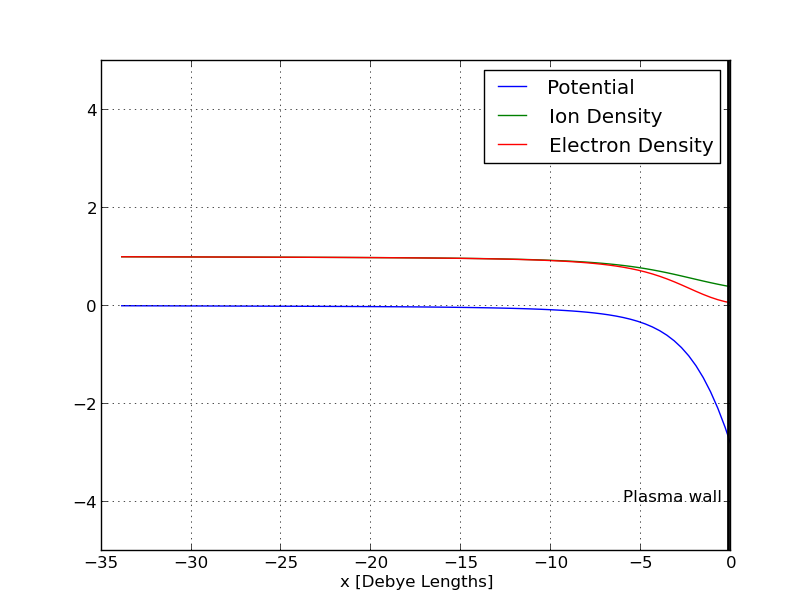
\includegraphics[width=0.8\textwidth]{graphofpotentialanddensity}
%\caption{Analytical solution of Poisson's equation for a planar sheath.}
%\label{fig:numericalsolution}
%\end{figure}
%This shows a sheath region of positive space charge a few Debye lengths thick. Before entering the sheath the density of the electrons is equal to that of the ions and the plasma potential is constant as the charge from the wall is screened out. A potential drop occurs in the sheath region as screening of the wall potential becomes less effective, reaching a maximum at the wall.
%
%The thickness of the sheath depends on the assumed boundary conditions therefore a plane sheath does not have a unique thickness. The sheath edge conditions are  arbitrary and these control the sheath thickness. There is a current dispute as to where the sheath edge should be chosen \cite{0963-0252-18-1-014004}. 
%The overall role of the sheath is to protect the wall from the plasma heat. Although the ion flux to the wall is increased by a factor of two by the presence of the sheath, the electron flux is reduced by a factor of 20 giving an overall reduction in flux of around an order of magnitude \cite{picmaster}.
%%http://www.en-trust.at/eibl/wp-content/uploads/sites/3/2013/08/Eibl05_MSc_thesis_physics.pdf
\section{Ideal Probe Theory}     \label{Section:Ideal}
The method for obtaining probe data is relatively simple. The probe is immersed in plasma and then biased to a potential ($V_B$) by an external circuit. The collected current ($I_p$) is then recorded at different probe voltages allowing an IV curve to be produced. The plasma parameters are then deduced from this IV characteristic. Charged particles are drawn to the probe by the surrounding electric field which extends a few Debye lengths into the plasma, in the sheath region. The theory developed by Langmuir and Mott-Smith allows the plasma parameters to be deduced for unmagnetised plasmas with a Maxwellian distribution of ions and electrons. This theory will be discussed before moving on to fusion relevant plasma conditions. 


When a probe is inserted into a plasma it is bombarded by neutral particles and the charged electrons and ions. Absent of any electric forces, the impact rate per $m^2$ for each species is given by their random thermal flux ($\Gamma$) which can be expressed as 
\be 
\Gamma_s = \frac{1}{4} n_s \langle{v_s}\rangle 
\label{eq:thermalmotion}
\ee
where $n_s$ is the number density of that particular species and $\langle{v_s}\rangle$ the average speed. For a Maxwellian distribution of particles this can be expressed as 
\be 
\Gamma_s =  \frac{1}{4} n_s \sqrt{\frac{8 k T_s}{\pi m_s}}
\ee
During probe operation, the probe voltage is swept from negative to positive while the current collected by the probe is recorded in order to produce the IV curve. Data for the entire curve is typically obtained in microseconds but this can be reduced. Advanced probe techniques are capable of completing a voltage sweep in $\approx 10^{-8}$ s \cite{time-res}. The current collected by the probe will be composed of ions or electrons or a combination of both depending on the applied potential of the probe. For $V_B = V_F$, no net current is drawn from the plasma as the electron flux reaching the probe is balanced by the ion flux. For $V_B > V_F$ the electron flux exceeds the ion flux and therefore a net current will flow into the plasma while for $V_B <V_F$ the ion flux exceeds the electron flux therefore a net current flows out of the plasma. For this report the sign convention declares current entering the plasma as a negative current and current leaving the plasma as positive current. A typical ideal IV curve is shown in figure \ref{fig:IV}. The curve is described as ideal because it is a theoretical prediction of an IV curve in an unperturbed plasma. Experimental IV curves deviate from the ideal case, as will be discussed.

%\begin{figure}[H]
%\centering
%\includegraphics[width=0.8\textwidth]{idealcurve}
%\caption{A theoretical IV curve that would be obtained by a Langmuir probe in an ideal plasma}
%\label{fig:idealcurve}
%\end{figure} 
\begin{figure}[H]
	\centering
	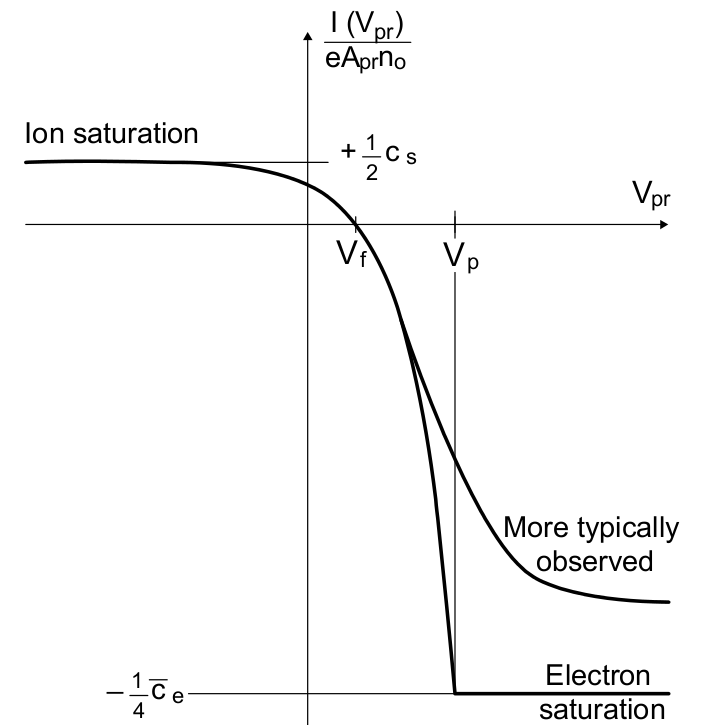
\includegraphics[width=0.8\textwidth]{monkiv}
	\caption{A schematic of the IV curve obtained with a single Langmuir probe \cite{monk}.}
	\label{fig:IV}
\end{figure}

%http://iopscience.iop.org/0741-3335/37/11/011/pdf/0741-3335_37_11_011.pdf

If no bias voltage is applied to the probe, the probe is allowed to float and will quickly charge up negative until it reaches the floating potential $(V_F)$. At floating potential the probe collects zero net current from the plasma. The floating potential is labelled on figure \ref{fig:IV}. It is less than the plasma potential ($V_{p}$) as a negative bias is required to retard the flow of electrons and accelerate ions in order to balance the two fluxes.  While $V_B < V_{p}$ the probe is biased negatively with respect to the plasma potential therefore ion collection to the probe is unhindered and so ions are collected at a saturated rate. If the probe bias is sufficiently negative all electrons are repelled and the current collected by the probe is then the ion saturation current approximated by the Bohm current 
\be 
I^{+}_{sat} = n_{i,sheath} e c_s A 
\label{eq:isat}
\ee
where $n_{i,sheath}$ is the ion density at the sheath edge, $e$ is the fundamental charge and $A$ the area of the exposed probe tip.
% This current arises due to the acceleration of the ions in the presheath. Equation \eqref{eq:presheathdrop} shows a decrease in the ion density at the sheath edge from that in the bulk plasma, we can therefore rewrite the ion saturation current in terms of bulk plasma parameters
%\be
%I^{+}_{sat} \approx 0.61 n_0 e v_B A
%\ee
%There are other theories for ion collection that allow the ion current to be calculated, these will be discussed later in the report. 
The ion flux is independent of the applied potential so making the probe more negative will not result in an increase in probe current. % Having said that under some conditions the sheath will expand as probe voltage becomes more negative this increases the collection area of the probe and so the ion current does not saturate. This will be discussed further when we look at probes in real conditions.

As the bias voltage increases (becomes more positive), the sheath potential drop is reduced allowing electrons at the high energy tail of the distribution to reach the probe. This region of the curve is known as the transition region. As $V_B \to V_{p}$ more and more electrons are able to reach the probe as less kinetic energy is needed to overcome the potential. For a Maxwellian distribution of electrons and neglecting effects such as secondary electron emission, the electron current able to reach the probe in the transition region is given by 
\be  
I^{-} = \frac{1}{4} n_0 e A \sqrt{\frac{8 k T_e}{\pi m_e}}  \exp\left[\frac{e(V_B-V_{p})}{k T_e}\right]
\label{eq:ecurrent}
\ee
The term $\sqrt{\frac{8 k T_e}{\pi m_e}}$ will be denoted as $c_e$ from now on. This is just the random thermal flux of the electrons reduced by the Boltzmann factor. The total current reaching the probe in this region will be made up of ions and electrons. At $V_B$ = $V_F$ the net current to the probe is zero, $I^+ = I^-$. By equating equation \eqref{eq:isat} and equation \eqref{eq:ecurrent} a value for the floating potential is found
\be 
V_f = V_{p} - \frac{k T_e}{2 e} ln\left[\left((2 \pi\frac{m_e}{m_i}\right)\left(1+\frac{T_i}{T_e}\right)\right]
\label{eq:floating}
\ee
In a pure hydrogenic plasma $V_f$ is typically found to be $\approx -3T_e $ V relative to the plasma potential.            %The total current as a function of bias voltage is then 
%\be 
%I(V_B) = - n_0 e A\left(0.61 v_B - \frac{1}{4}  c_e \exp\left[\frac{e(V_p-V_{p}}{k T_e}\right] \right)
%\ee
As the probe bias continues to rise it will eventually be equal to the plasma potential. At this point there is no potential difference between the probe and the plasma, therefore there are no electric fields and so the sheath disappears. The charged particles now reach the surface of the probe due to their thermal motion and so the probe collects the thermal flux of both electrons and ions. No electrons are repelled any more. Increasing the potential of the probe will act to repel the ions and a negative sheath of electrons now forms around the positive probe to shield out the positive charge. This sheath is very thin and the electric field outside of it is again zero. If the probe bias is sufficiently positive, no ions can reach the probe and the probe collects the electron saturation current. This is just the random thermal flux of electrons that enter the sheath
\be  
I^{-}_{sat} = \frac{1}{4} n_0 e c_e A
\label{eq:esat}
\ee
For a pure hydrogenic plasma, with no magnetic fields, the ratio of the electron saturation current to ion saturation current is given by
\be 
\frac{I^{-}_{sat}}{I^{+}_{sat}} \approx 60
\ee
Therefore, at bias voltages where $V_B > V_{p}$, the ion contribution to the total current is negligible. For this reason Langmuir probe measurements cannot be used to determine the ion temperature. %the ion contribution to the total current is negligible and often ignored. The total current reaching the probe when $V_B > V_{p}$ is then given by \eqref{eq:esat}. %An increase in the saturation current is noticed with increased applied voltage due to the sheath around the probe expanding. This acts to increase the effective collecting area of the probe. The shape of the resulting curve depends on the shape of the exposed probe tip. GET REFERENCE

%he curve has a sharp knee at this point where the collected current is no longer exponentially increasing. This sharp knee is often rounded in experimental curves.
Once the probe has been swept an I-V curve can be constructed. In the transition region, the electron current contribution ($I^-$) can be obtained by deducting the ion saturation current from the total current. By rearranging equation \ref{eq:ecurrent} it can be seen that 
\be
\ln(I^-) = \ln(I^-_{sat}) + \frac{e(V_B-V_p)}{kT_e}
\ee
The electron temperature can than be obtained by plotting $ln(I^-)$ against $V_B$, the inverse of the gradient giving $T_e$ in eV. Once $T_e$ is known, the plasma density can be extracted from the measurement of the ion saturation current, using equation \ref{eq:isat}. This does require a measurement of $T_i$ , which is not possible to measure using a standard Lamguir probe. Often the assumption of $T_i = T_e$ is used, the validity of this assumption is assessed in section \ref{Section:assumption}. As well as Retarding Field Energy analysers discussed in section \ref{Section:assumption}, other advanced probe techniques have been to developed to measure $T_i$, these are discussed in section \ref{Section:advanced}.
Floating potential measurements can be made directly by not biasing the probe or can be inferred from the IV curve as shown in figure \ref{fig:IV}. In theory the plasma potential can also be read from the IV curve, characterised by the sharp knee. However, in practise, the knee is rounded and so equation \ref{eq:floating} is used to determine $V_p$.
The above equations have all assumed the simplest case of a collisionless sheath with no magnetic field present. All plasma-surface interactions have been neglected. IV curves obtained in tokamak plasmas differ from figure \ref{fig:IV} because these assumptions are not always valid. The magnetic field has a strong influence on the dynamics of charged particles and hence the collection of those particles by the probe. The effects of a magnetic field on probe interpretation is discussed in section \ref{Section:magnetised}. %Also these equations are only valid for the thin sheath regime where the probe diameter $d$ $>>$ $\lambda_D$. In some cases (list) it is possible for a thick sheath regime to exist. In this case $\lambda_D >> d$. Due to their orbital motions around the probe, not all charged particles that enter the sheath will actually be collected by the probe. The current drawn by the probe is now a function of bias voltage and also depends on the detailed geometry of the probe. 
\section{The Pre-sheath in Magnetised Plasmas}
% Really good overview https://arxiv.org/pdf/1509.04479.pdf
For an unmagnetised plasma, the boundary layer between the plasma and a contacting surface consists of a quasi-neutral pre-sheath, which acts to accelerate ions up to the Bohm speed, and the Debye sheath where quasi-neutrality no longer holds. Often in experimental plasmas, such as tokamak experiments, a magnetic field is applied to the plasma to aid in confinement. The presence of the magnetic field affects particle dynamics and changes the constitution of the boundary layer. A numerical model was developed by Chodura \cite{Chodura} to study the effect of an oblique magnetic field, where the angle ($\alpha$) between the field and the tangent to the surface satisfies $\alpha \neq 90^\circ$. It was found that  there exists three distinct regions between the bulk plasma and the material surface as shown in figure \ref{fig:MPS}. The first region is the familiar pre-sheath which extends far into the plasma. The second region is the Magnetic Pre-Sheath (MPS) which is also quasi-neutral. The size of the MPS scales with the ion Larmor radius and is influenced by the angle between the magnetic field and the surface normal. There is no MPS at normal incidence. The final layer is the familiar electrostatic Debye sheath where quasi-neutrality breaks down. 
\begin{figure}[H]
	\centering
	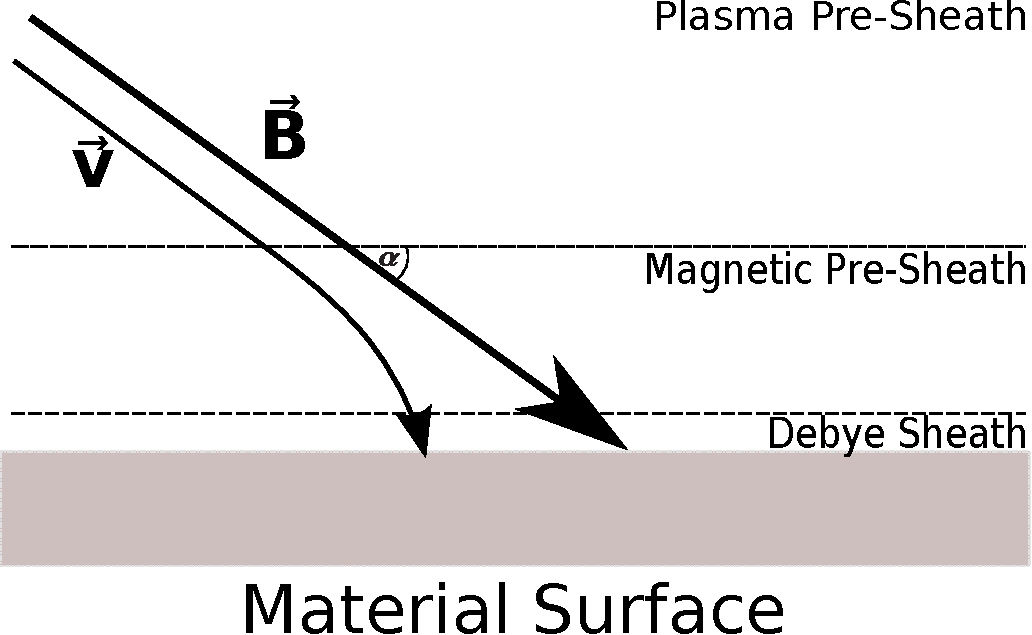
\includegraphics[width=0.8\textwidth]{magnetic_pre_sheath.pdf}
	\caption{The structure of the sheath in front of a material surface in a magnetised plasma. Particles enter the magnetic pre-sheath with parallel velocity exceeding the Bohm velocity. In the magnetic pre-sheath the particles velocity is turned so that it is sonic perpendicular to the surface on entrance to the Debye sheath. }
	\label{fig:MPS}
\end{figure}


Chodura found that the role of the pre-sheath in a magnetised plasma is to accelerate ions such that their parallel velocity along the field lines ($v_{\parallel}$) exceeds the Bohm speed on entering the MPS. This is known as the Bohm-Chodura criterion 
\begin{equation}
v_{\parallel} \geq c_s
\end{equation}
Chodura also discovered that the ions velocity was turned from being sonic parallel to the field lines on exiting the pre-sheath to being sonic normal to the surface at the Debye sheath entrance. The role of the MPS is to turn the flow of ions so that they satisfy the Bohm Criterion on entrance to the Debye sheath. The mechanism for this depends on the presence of an electric field in the MPS, the gradient of which results in a polarisation drift \cite{MPS_polarisation}. A potential drop ($V_{MPS}$) across the MPS region is responsible for the electric field. The magnitude of this potential drop depends on the angle of attack \cite{stangeby-angles}
\be 
V_{MPS} = -\frac{kTe}{e} \ln(\sin\alpha) 
\ee  
The total potential drop ($V_f$) between the plasma and wall, however,  does not depend on the presence of the magnetic field and so the floating potential of an object in a magnetised plasma is still given by equation  \ref{eq:floating}. The total potential drop is the sum of the potential drop across the MPS and the potential drop across the Debye sheath ($V_{DS}$)
\be
V_f = V_{MPS} + V_{DS}
\ee

 It was realised by Stangeby \cite{stangeby-angles} that for increasingly lower values of $\alpha$, the potential drop across the MPS grows until a critical angle is reached ($\alpha_c$), at which point $V_{MPS} = V_f$. For a deuterium plasma, with $T_e = T_i$, $V_f = 2.84$. The MPS potential drop will become equal to this once $\alpha \leq \alpha_c =  {3.35}^{\circ}$. The potential drop in the MPS represents the change in potential required to turn the ion flow from being sonic parallel to the field lines, to sonic normal to the surface. For small $\alpha$, there is not enough potential drop across the MPS available to turn the ions towards the surface, the ions therefore exit the MPS with a subsonic velocity normal to the surface. This regime is relevant to fusion devices, with angles of incidence as low as ${1}^{\circ}$ reported in C-mod \cite{c-mod}. Stangeby hypothesised the disappearance of the Debye sheath for angles of incidence below the critical angle. This hypothesis was confirmed by kinetic simulations \cite{kinetic-sims}. For these angles, the electron current to the wall is limited by the magnetic field, with electrons tied to the field lines, whilst the larger ion Larmor radius allows ions to reach the wall more readily. An ambipolar flow to the wall can be maintained without the need for a strong ion acceleration and so the Debye sheath is unnecessary. In extreme cases where $\alpha < \left({\frac{m_e}{m_i}}\right)^{0.5}$, the larger orbit of the ions means they are the more mobile species, reaching the wall faster and causing it to charge up positively. A more complex sheath arises in this case. The angle at which this would occur in a deuterium plasma is $\approx \alpha < {1}^{\circ}$. This regime is currently not applicable to fusion devices as it requires an extremely high degree of alignment of the divertor tiles but it may become relevant with future devices that strive to reduce $\alpha$ in order to minimise heat and particle flux density to the divertor.
 
 
 
% This is true until a critical angle near $\alpha \approx 0^\circ$ where the ions, due to their larger Larmor radius, reach the wall more quickly than the electrons, causing it to charge up positively. This leads to a more complex sheath behaviour \cite{MPS-Stangeby}.
\section{Probes in Magnetised Plasma} \label{Section:magnetised}
Fusion devices such as tokamaks use strong magnetic fields to confine the plasma long enough for fusion to occur. The presence of a magnetic field changes the dynamics of particles moving in the sheath and so has an impact on measurements made by probes. Probes are used at the edge of tokamaks to diagnose the plasma at the plasma-surface interface. It is important that the effects of magnetic fields on probe readings are understood in order to correctly interpret probe data.
The magnetic field restricts the motion of charged particles. They are free to stream along the field lines (parallel to B) but their cross-field motion is now restricted. Charged particles orbit the magnetic field lines in circular orbits with radius equivalent to the Larmor radius ($\rho_L$) given by
\be 
\rho_L = \frac{v m}{e B}
\ee
Where $v$ is the velocity of the charged particle, $m$ its mass and $B$ the strength of the magnetic field in Tesla.  In an unmagnetised plasma, the dynamics of charged particles are determined by the electric field of the plasma sheath and pre-sheath but with a magnetic field particles can no longer free stream to the probe.
The situation is now two dimensional as particles are restricted to following the magnetic field lines. Particle transport to the probe is now restricted by cross-field diffusion and the size of the probe starts to become important. 
The extent of how probe measurements are affected by the addition of a magnetic field depends on the relative size of the probe dimension $d$ to that of the Larmor radius. Due to their lower mass the electrons have a much smaller Larmor radius than the ions and so are affected more by the presence of a magnetic field. The probe is described to be in the weak field regime when $B$ is low enough such that
\be
\rho_{L,ion} > \rho_{L, electron} > d
\ee
In this regime particles are still able to intercept the probe as they orbit the field lines and so particle collection is unaffected. The field free results from ideal theory as previously discussed should still apply. As the strength of the field is increased the Larmor radius decreases. Eventually the dimensions of the probe exceed the Larmor radius of the electrons such that 
\be
\rho_{L,ion} > d >  \rho_{L, electron}
\ee
this is known as the strong field regime. The ions with their larger mass are relatively unaffected by the magnetic field in this regime, on the other hand the collection of electrons to the probe is restricted as electrons are constrained to orbit the field lines. Electrons will only be collected by the probe if their field line ends on the probe itself, so flow to the probe is dominated by cross-field transport processes which allow charged particles to move from one field line to another. The flux of particles exiting the flux tube connected to the probe must be balanced by a flux of particles entering the flux tube via cross-field diffusion. It takes a long length of flux tube to balance the two fluxes because parallel transport along the field line occurs much faster than perpendicular transport. This length over which the fluxes become balanced is known as the probe collection length $L_{col}$ and is illustrated below.

\begin{figure}[H]
	\centering
	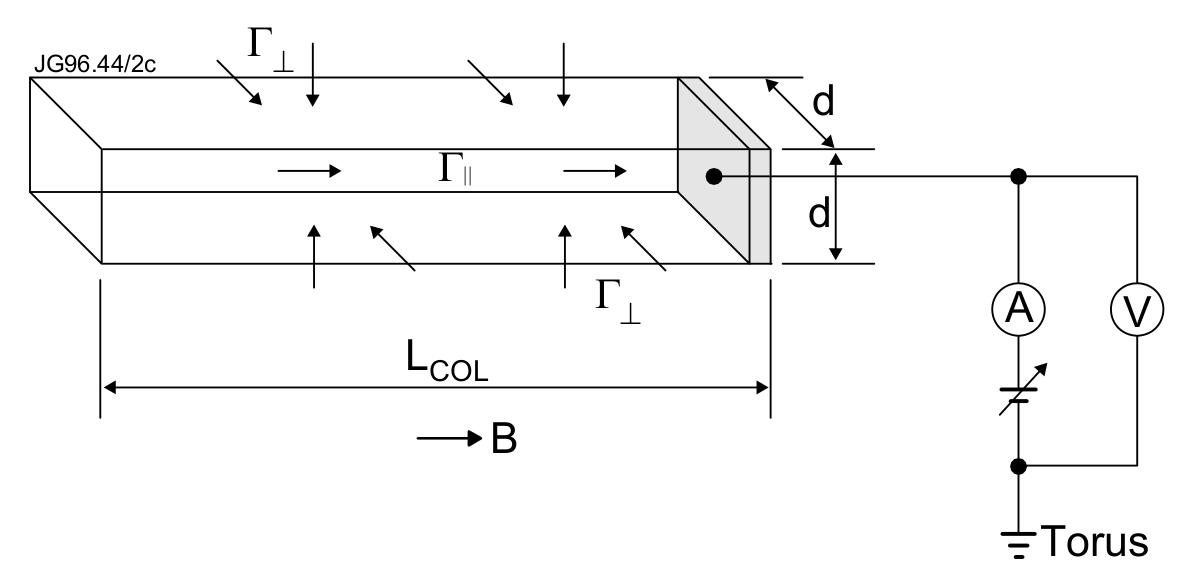
\includegraphics[width=0.8\textwidth]{collectionlength}
	\caption{The probe of dimension $d$ has a collection length associated with it ($L_{col}$) where $L_{col}>>d$ \cite{bias-probes}}
	\label{fig:shape}
\end{figure}

$L_{col}$ is a measure of the distance in which a probe disturbs the plasma it is in. During net electron collection the current drawn by the probe is higher, therefore the collection length increases to balance the higher parallel flux. %The collection length can expand to become greater than the connection length in the SOL, this will be discussed in more detail in the following section.
One consequence of the probe collection length is that measurements from the probe are no longer localised but are averaged over the entire collection length. Electron collection is no longer well described by the random electron flux equation \eqref{eq:esat} in a magnetised plasma. The most striking evidence that magnetic fields affect probe readings is from observing a dramatic reduction in the electron saturation current to ion saturation current ratio. Bohm predicted values as low as 10 \cite{discharges} and this was confirmed experimentally by Sugawara \cite{monk}. Values for this ratio have been recorded in tokamaks to be even as low as unity \cite{matthews}. IS THIS BECAUSE THE ELECTRONS ARE MAGNETISED BUT IONS NOT SO ELECTRONS ONLY SEE THE PROJECTED AREA, IONS SEE WHOLE AREA? In JET it was demonstrated that artificially high values of $T_e$ were obtained when fitting an exponential to regions of the IV curve where $V_B > V_F$ \cite{JET_TE}. However no significant change in $T_e$ was observed when using regions below the floating potential. It is now standard procedure to only fit the exponential to regions below the floating potential for probes in magnetised plasma. The more points that are used in the temperature fit from bias voltages greater than the $V_f$, the higher the measured temperature \cite{matthews}. The reason for this is attributed to collisions that occur between the electrons and ions along the collection tube. Regions of increased potential (potential hills) are required, both cross-field and parallel to the field, to attract electrons to the probe. As a result, ions in the probe flux tube find themselves in a retarding field and so obey the Boltzmann relation such that $n_i \propto \exp(-V/T_i)$. Therefore a density depression exists just in front of the probe. The electron current to the probe is proportional to the plasma density in front of the probe. A reduced plasma density results in a reduced electron current as compared to the unmagnetised case. The collisions between the ions and electrons constitutes a resistance in what is known as the probe circuit shown in figure \ref{circuit}.

\begin{figure}[H]
	\centering
	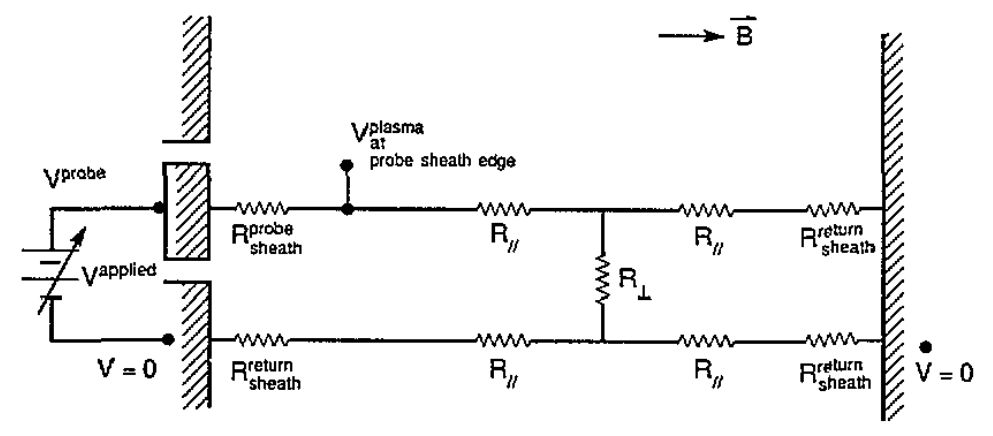
\includegraphics[width=0.8\textwidth]{sheathcircuit}
	\caption{There are various resistances associated with the probe circuit.\cite{te-determination}}
	\label{circuit}
\end{figure}
 %$R^{probe}_{sheath}$ is  given by
In an unmagnetised plasma the only source of resistance is the sheath resistance $R^{probe}_{sheath}$ and the return sheath resistance $R^{return}_{sheath}$. The return sheath completes the probe circuit and is located in between the plasma and the material wall bounding the plasma. The return sheath is present in any probe circuit. Single probe theory is a good approximation in the unmagnetised case provided that the collection area of the return sheath is much greater than the collection area of the probe sheath. If this is true it can be assumed that $R^{return}_{sheath} =0$ as resistance is inversely proportional to area. In the case when $B=0$ the area of the return sheath is essentially the surface area of the vessel wall and so this requirement is met. No other sources of resistance are present so the probe bias only appears across the probe sheath. If this is the case then the IV characteristic is defined by
\be 
I = I_{sat}^{+}  \left[1-exp ( \frac{(V-V_F)}{k T_e} ) \right]
\label{eq:resistance}
\ee 
where $V$ is the value of the voltage drop across the sheath. $V = V_B - V_s$ with $V_B$ being the applied probe voltage and $V_s$ the plasma potential at the sheath edge of the probe. With no other sources of resistance present, the entirety of the applied voltage to the probe is contained in the sheath and so $V_s = 0$. Adding a magnetic field introduces new sources of resistance including the parallel resistance $R_\parallel$ and perpendicular resistance $R_\perp$. The applied voltage to the probe is now shared between the probes sheath resistance and all other sources of resistance in the circuit and because of this it is no longer valid to assume $V_s = 0$. Without knowing the value for $V_s$ it is not possible to use \eqref{eq:resistance} to derive $T_e$. In principle it could be possible to model all the other sources of resistance within the circuit in order to calculate the probe-sheath resistance which would then give $V_s$ but cross-field transport mechanisms are not well understood.



$R_{\perp}$ is the resistance associated with cross field transport and could have different values for ions and electrons. It can not be modelled due to the lack of understanding of cross-field transport mechanisms. $R_{\parallel}$ is the resistance associated with parallel transport. Sources include friction caused by collisions with neutral particles and friction between the oppositely charged electrons and ions. The inability to model perpendicular resistance also prevents us from modelling the two other resistances in the circuit. $R^{return}_{sheath}$ depends on the area of the return sheath which in turn depends on the ratio of parallel to perpendicular transport. This ratio also determines whether or not the probe circuit extends to the other divertor target or closes back on itself. The path it takes will impact the parallel resistance. Because these resistances cannot be modelled it is not possible to calculate the value of $V_s$ unless $R_{sheath}^{probe} >> R$ where $R$ is all other forms of resistance in the circuit. If this is the case, single probe theory can be used to extract $T_e$ when the plasma is magnetised. 

% To summarise the problems so far. The electron current is strongly distorted by the presence of a magnetic field as demonstrated by the low electron saturation current observed in experiments. The electron saturation region is not often used in experiments as the high particle flux would cause the probe to melt and so it may appear as though a low saturation current isn't really a problem. However it has been shown in JET that the electron current increases more slowly than expected for all points above the floating potential. This means that as more points are included from the region of net electron collection the value of the derived electron temperature increases. It may be possible to limit analysis of probe data to just that collected below the floating potential where the probe is predominately collecting ions which are relatively unaffected by presence of a magnetic field. However by doing this the derived electron temperature is based only on the high energy tail of the electron distribution which is capable of reaching the negative probe, if this distribution isn't Maxwellian the electron temperature will be overestimated. It is also sometimes necessary to include points from the electron collection region when dealing with noisy data otherwise statistical noise begins to dominate the results. Without knowing the additional circuit resistances it is not possible to use \eqref{eq:resistance} to derive $T_e$ as assuming the potential at the probe-sheath edge is zero will lead to overestimating the electron temperature.

Naturally the question arises - can Langmuir probes be used reliably in magnetised plasmas? Experiments with a pin-plate probe were conducted to test if the portion of the IV curve below floating could be used safely to derive $T_e$ \cite{pin-plate-pitts}. The pin-plate probe consisted of a Langmuir probe plate, with dimensions 10 mm x 5 mm and a pin probe of diameter 1 mm and a length of 5 mm, placed 2.5 mm in front of the plate. The pin was operated in floating mode for the duration of the experiment whilst the plate probe was swept as with a standard Langmuir probe. A schematic of the pin-plate probe is shown in figure \ref{fig:pin_plate_probe}. The floating potential of the pin was representative of the plasma potential outside the plate sheath, offset by a factor assumed to be constant. The experiments found that the potential on the floating pin remained almost constant for bias voltages on the plate that satisfied $V_B^{plate}  <V_F^{plate}$. It can be concluded from this that for these bias voltages, the plate potential was entirely contained in the plate sheath and so  $R_{sheath}^{probe} >> R$. As a result $T_e$ can be extracted safely from this region. There was a slight increase of a few volts once $V_B$  was within a few $T_e$ of floating i.e. $V_F - 3 T_e \leq V_B \leq V_F$. This was attributed to either an extraneous effect or some of the probe bias appearing elsewhere in the probe circuit. If the later were true, the paper expects between a $15 \% \to 20\%$ error in the $T_e$ measurement when using this region. For bias voltages such that  $V_B^{plate} > V_F^{plate}$ it was found that the pin floating potential increased monotonically with the bias voltage applied to the plate. This is due to the formation of a potential hill which is established to drive the electron current to the probe against the friction of the ions in the probe collection tube. This potential hill results in a reduced plasma density in front of the probe which leads to a reduced electron current. The electron current in this region no longer behaves as a simple exponential. Including points from this region in the exponential fit will result in a spuriously high measurement of the electron temperature. In later work, Stangeby concluded that it is a reasonable assumption to use the region of the IV curve below floating potential to yield a reliable value of $T_e$ \cite{pin-plate-stangeby}.

\begin{figure}[H]
	\centering
	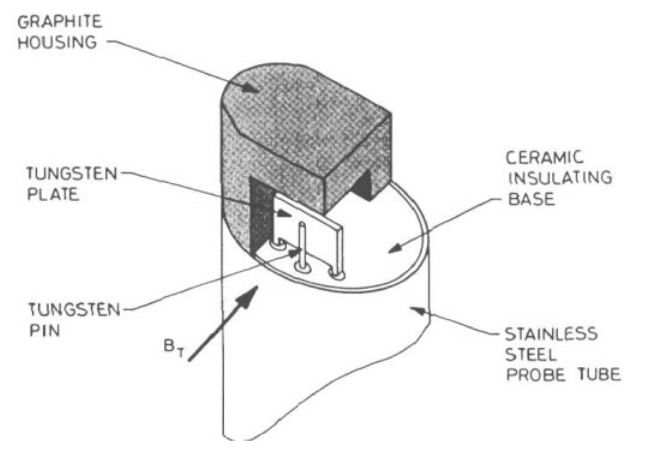
\includegraphics[width=0.8\textwidth]{pin_plate_probe.png}
	\caption{The pin-plate probe consisting of a tungsten pin located in front of a tungsten plate.  \cite{pin-plate-stangeby}.}
	\label{fig:pin_plate_probe}
\end{figure}


 %Two models exist that are capable of explaining the distortion to the electron collection region of the IV curve, the Bohm-Cohen-Stangeby (BCS) model and Gunther's model. 

%\subsubsection{BCS Model}
%This model is based on the work of Bohm in 1949 \cite{discharges}. During net electron collection the collection length of the probe extends to balance parallel and perpendicular transport into the flux tube. The collection length becomes so long that it exceeds the mean-free-path for electron-ion collisions and so the electrons lose momentum to ions as they are drawn along the long flux tube to the probe. An electric field is established in order to drive the electron current against the resistance from the collisions. The probe acts as a sink for electrons, draining the plasma in front of it and hence a parallel density gradient is set up. This also acts to drive the electron flux along the flux tube which can be expressed as 
%\be
%\Gamma_\parallel = -D_\parallel \frac{dn}{dx} + n \mu_\parallel E 
%\label{eq:parallelflux}
%\ee
%where $E = - \frac{dV}{dx}$ is the electric field, $\mu_\parallel$ the electron mobility coefficient along $\vec{B}$ and $D_\parallel$ the electron diffusion coefficient along $\vec{B}$.
%$\mu_\parallel$ and $D_\parallel$ are related to each other using the Einstein relation 
%\be 
%\frac{D_\parallel}{\mu_\parallel} = -\frac{kT_e}{e}
%\ee 
%%Equation \eqref{eq:parallelflux} can now be expressed as 
%%\be 
%A similar relation exists for the perpendicular flux entering the flux tube but the perpendicular diffusion coefficient $D_\perp$ is anomalous. 
%\be
%\Gamma_\perp = -D_\perp \frac{dn}{dx} + n \mu_\perp E 
%\label{eq:perpflux}
%\ee
%The electron collection length can be determined by equating equations \eqref{eq:parallelflux} and \eqref{eq:perpflux}. This allows the parallel flux to be rewritten as 
%\be
%\Gamma_\parallel = \frac{2D_\parallel (1+\tau)(n_0 - n_1)\sqrt{\alpha}}{d}
%\ee 
%Where $\tau = \frac{T_i}{T_e}$ , $\alpha = \frac{D_\perp}{D_\parallel}$ and $d$ is the probe dimension. %WHAT IS NO AND N1.  
%It is found that the electron saturation current is reduced by a reduction factor $r$ 
%\be 
%I^i_{sat} = \frac{1}{4} n_0 e c_e A_\perp \left(\frac{r}{1+r}\right) 
%\ee
%Where $r$ is defined as 
%\be 
%\frac{16}{\pi} \frac{\lambda \sqrt{\alpha} (1+\tau)}{d}
%\ee
%With $\lambda$ the electron mean free path. $\alpha$ decreases as the magnetic field strength increases therefore for large B $r << 1 $ and so 
%\be 
%I^i_{sat} \approx \frac{1}{4} n_0 e c_e A_\perp r 
%\ee
%This reproduces the zero field case as $B \to 0$. The physical explanation for the reduced electron current in this model is the electron flow to the probe is restricted due to the momentum they lose to the ions. When biased below the floating potential to collect ions momentum loss to the electrons can be ignored so this region of the curve may still be usable \cite{matthews}. The downside to this model is that cross-field transport is not well understood and so it is not known what value $D_\perp$ should have. 
%The electric field set up to drag the electrons to the probe also repels the ions. 



% However as long as the probe is biased negatively so that it is repelling electrons, their density can still be well described by the Boltzmann factor. $T_e$ can therefore still be derived successfully by restricting the IV characteristic up to the floating potential.








Once a probe is operating in the strong regime, the effects of the magnetic field must be taken into account in order to reliably measure the electron temperature. Increasing the field further leads to the 'very strong field' regime. This is defined at the point where
\be
d > \rho_{L,ion} >  \rho_{L, electron}
\ee
The motion of both electrons and ions is now strongly affected by the field. It is simple to see whether or not this regime is relevant to fusion. As a typical example the field in the divertor region of JET is  $\approx 3T$ and the electrons and ions have a temperature of around $10eV$. This gives the ions a Larmor radius of $\approx$ $0.1mm$ while probes are typically $2mm$ long. The high temperatures in this region place a constraint on the size of the probes as they need to be large enough to dissipate the heat and avoid being melted, so making the probes smaller in order to simplify probe interpretation is not a viable option. 
In this regime, particles are only able to reach the probe from the direction parallel to the field so it appears to them that the probe has a plane geometry regardless of its actual geometry. This means the effective collection area of the probe ($A_{eff}$) is now reduced from its actual surface area ($A_{surface}$) to the projection of the surface ($A_{proj}$) in the direction of the field 
\be
A_{eff} = A_{proj} = A_{surface} sin(\theta)
\ee
where $\theta$ is the angle between the field and probe as shown in figure \ref{fig:proj_area}.
The shape of the probe in this regime is not very important only its cross sectional area perpendicular to $\vec{B}$ \cite{te-determination}. As demonstrated by equation \ref{eq:isat}, the effective collection area of the probe must be known in order to determine the plasma density from measurements of the ion saturation current. Experiments were carried out by Brown in a linear plasma device that contained two sets of diagnostics capable of measuring the electron density, Langmuir probes and a microwave interferometer \cite{probe-response}. Both diagnostics were used simultaneously whilst the magnetic field strength was increased. As the field became stronger, the electron density derived from probe readings deviated from those obtained by the interferometry. The probes gave a lower value of $n_e$ than measured by the interferometry. This can be explained by a reduction in the collection area of the probe due to the increased field which then results in a lower value for $I_{sat}^+$. If the effects of the magnetic field are not taken into account the plasma density will be underestimated and the electron temperature overestimated.
\begin{figure}[H]
	\centering
	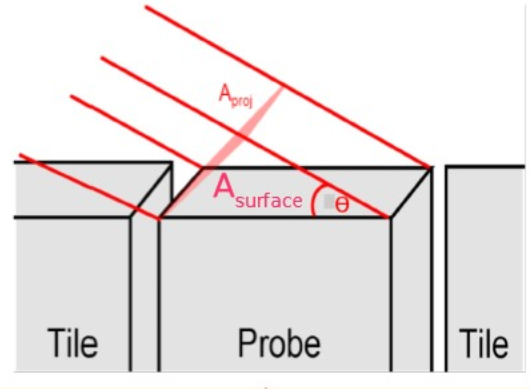
\includegraphics[width=0.8\textwidth]{projected_area.PNG}
	\caption{In a strongly magnetised plasma the effective collection area of the probe is reduced from its surface area ($A_{surface}$) to the projection of that surface perpendicular to the magnetic field ($A_{proj}$). }
	\label{fig:proj_area}
\end{figure} 
\section{Langmuir Probes in Tokamaks}

A tokamak plasma with high temperature and density is a hostile environment for a material surface. Any material placed into the plasma, such as a probe, will suffer damage from the high heat and particle flux impinging on it. This is also true of probes placed in the relatively cooler and less dense SOL region. Steps have to be taken to ensure the probes survive the plasma conditions so that useful measurements can be taken. It is also important that the probe does not contaminate the plasma, particularly with high Z impurities which reduce the temperature of the plasma by radiative cooling. Various techniques have been developed to enhance the lifetime of tokamak probes. One technique is to place the probes in a reciprocating probe head. This head can be submersed into the SOL via a drive mechanism which is connected to a support structure. The drive mechanism plunges the head into a region of the SOL, the probe then takes its measurements before being retracted back into the vacuum region away from the plasma. An additional benefit of reciprocating system is that it allows the probe to measure different depths of the SOL plasma, allowing SOL profiles to be constructed. The probe head may be exposed to plasma for $\approx$ 100 ms during a typical plunge. It is advantageous for the probe head to be as light as possible so that it can be quickly accelerated into and out of the plasma. It must also be able to survive heat fluxes on the order of 10 MW/m$^2$ \cite{first_wall}. Graphite is the material of choice in many tokamaks as it is a low Z material capable of withstanding the hostile conditions presented by the plasma. Low Z impurities result in less cooling to the core due to radiative cooling. However, over time, damage to the probe is inevitable. Modular designs are often employed on modern tokamaks to aid in the task of probe replacement. Another technique is to use heat sink probes that are in good thermal contact with a large heat sink.

An alternative probe design is to align the probe so that its surface is flush with the surrounding divertor tiles. These Flush Mounted Probes (FMP) are one of the most robust probe designs and they are almost as resilient as the divertor tiles, sharing the same geometry relative to the magnetic field \cite{FMP-intro}. The grazing angle between the field and the FMP in the divertor region means the intense heat flux is spread out over a larger area thus reducing the damage to the probe. This grazing field line can lead to complications in interpreting the data obtained from FMPs as the projected area of the probe can become comparable to the sheath area for such small field line angles. This will be discussed further in Chapter X.


\section{Underlying Assumptions of Probe Theory}
\label{Section:assumption}
In deriving the equations of section \ref{Section:Ideal} it was assumed the particles had a Maxwellian velocity distribution. A reciprocating probe was used on COMPASS to evaluate the velocity distribution of electrons within the last closed flux surface (LCFS) and the SOL. Within the LCFS and SOL, evidence for a bi-Maxwellian distribution of electrons was found, corresponding to two Maxwellian distributions of electrons at different temperatures \cite{bi-max}. This has also been reported on CASTOR \cite{castor-bi} and NSTX \cite{nstx-bi}. This can lead to errors in the electron temperature measurement, especially if the I-V curve is only swept up to the floating potential, in which case only the high energy tail of the electron distribution is sampled. In the far SOL, close to the walls it was found that the electrons adopted a single Maxwellian distribution and so the assumption was valid in this region of the tokamak.
A value for $T_i$ is required to obtain the plasma density from the ion saturation current. Due to difficulties in obtaining a measurement for this value it is often assumed to be the same as the measured $T_e$ value. Retarding Field Energy Analysers (RFEA) can be used to obtain measurements of $T_i$, by using a series of charged plates and grids to repel electrons and only collect the ions. The exponential drop off of the ion current, as the bias voltage is swept, can then be used to extract $T_i$. Two RFEAs were placed on MAST to measure the ion temperature \cite{sarah}.It was found that for low power L-mode plasma discharges, $T_I = T_e$ was a good assumption at the target and in the SOL. However, for higher power discharges and in H-mode, ratios of $T_i/T_e = 1 \to 3$ were observed so this assumption may not always hold.
%http://www.seas.ucla.edu/~ffchen/Publs/Chen210R.pdf 

%Close to the target this is a good approximaton " It is shown that close to the wall of the
%tokamak chamber the energy distribution function of the electrons is Maxwellian," 

%http://iopscience.iop.org/article/10.1088/1742-6596/514/1/012049/pdf

%Probe theory based on assumptions, one electron temp present, Maxwellian distributed. Test these assumptions
%Ti = Te  , discuss this, RFEA's what does Sarah's thesis say about this assumption? 
%"
%In the absence of data for the ion temperature it is assumed that T i = T e when
%deducing such values as the electron density, n e , and power to divertor, P div , from
%Langmuir probe data using j sat measurements. This assumption needs investigating
%since the few measurements which have been made in the SOL at the midplane of
%tokamaks has given T i /T e to be between 1.5 and 10 [14] and this can lead to the
%overestimation of n e by over a factor of 2 [49]." 


%"For these low power L-mode plasma discharges,
%T i ∼ T e is a good assumption at the target in both the SOL and the private flux
%region on MAST."  
%
%
%i /T e ∼ 2 at the target has been measured constantly across divertor
%target profiles for higher power discharges, achieved through additional neutral beam
%heating 
%
%
%Measurements have been made of the ion temperature at the divertor in inter-ELM
%H-mode and have shown that across a radial target profile T i = 6−20 eV with T i /T e
%= 1−3 over a range of plasma parameters. 

%How much error does a ratio of 3 bring about?


\section{Advanced Probe Designs}
\label{Section:advanced}
A whole range of advanced probe techniques have been developed in order to measure quantities such as the plasma potential, electron temperature, electron density and ion temperature without the limitations of standard Langmuir probes discussed above.  Ball-pen probes and emissive probes aim to measure the plasma potential directly by reducing the ratio of the saturation currents to one such that the probe floats at the plasma potential \cite{advanced}. These will be discussed in Chapters X and Y respectively. BPP's and LP's can be used simultaneously to provide fast measurements of $T_e$, this will also be discussed in Chapter X. 
A segmented tunnel probe has been developed that is capable of measuring the electron temperature without actually collecting any electrons \cite{tunnel}. The probe is U-shaped, consisting of a conducting tunnel and a conducting backplate. Both conductors are biased sufficiently negatively to repel all electrons. The ion current collected by each conductor is measured. The ratio of the currents to each collector depends on the thickness of the sheath at the entrance to the tunnel which in turn depends on $T_e$. This relationship is derived from Particle-In-Cell modelling of the probe. By adding a conducting diaphragm around the entrance to the tunnel it is possible to prevent electrons from reaching one of the tunnel segments \cite{tunnel_ti}. By sweeping the bias voltage across this segment, an exponential fall off in the ion current is observed. This data is hidden by the electron current for a standard probe. The rate at which the ion current decreases allows $T_i$ measurements to be made. The segmented tunnel probe is one example of a family of probes that aim to shield the electrons from a collector so that the ion current can be analysed. These Ion Sensitive Probes (ISP) often exploit the difference in Larmor radii of the electrons and ions to inhibit electrons from reaching a part of the probe \cite{review_isp}. 
%As has been discussed, a Langmuir probe floats negatively with respect to the plasma potential due to the higher mobility of the electrons compared to the ions. From equation \ref{eq:floating}, it can be seen that this offset from the plasma potential depends on the mass ratio of the electrons and ions and their respective temperatures $T_e$ and $T_i$. The plasma potential is an important quantity, measurements of it are vital for modelling transport phenomena in the edge region of tokamaks. 


\section{Summary}
Sheath theory has been introduced as this underpins measurements made by electric probes in plasmas. Standard Langmuir probe theory has been introduced and complications in probe interpretation arising from the presence of magnetic fields have been discussed, this will be explored further in chapter X. Various advanced probe techniques have been summarised, of these the BPP and emissive probe will be studied in chapter Y and Z respectively. 

\section{References}
\bibliography{references}
\end{document}